\documentclass[aps,pra,preprint,groupedaddress]{revtex4-1}
%\documentclass[aps,prl,preprint,superscriptaddress]{revtex4-1}
%\documentclass[aps,prl,reprint,groupedaddress]{revtex4-1}

\usepackage{graphicx}
\usepackage{amsmath}

% You should use BibTeX and apsrev.bst for references
% Choosing a journal automatically selects the correct APS
% BibTeX style file (bst file), so only uncomment the line
% below if necessary.
%\bibliographystyle{apsrev4-1}

\begin{document}

\title{Phase Dependent Ionization of Rydberg Atoms in Static Fields}

% repeat the \author .. \affiliation  etc. as needed
% \email, \thanks, \homepage, \altaffiliation all apply to the current
% author. Explanatory text should go in the []'s, actual e-mail
% address or url should go in the {}'s for \email and \homepage.
% Please use the appropriate macro foreach each type of information

% \affiliation command applies to all authors since the last
% \affiliation command. The \affiliation command should follow the
% other information
% \affiliation can be followed by \email, \homepage, \thanks as well.
\author{Eric Magnuson}
\email[]{edm5gb@virginia.edu}
\author{Tom Gallagher}
%\homepage[]{Your web page}
%\thanks{}
%\altaffiliation{}
\affiliation{University of Virginia, Department of Physics}

%Collaboration name if desired (requires use of superscriptaddress
%option in \documentclass). \noaffiliation is required (may also be
%used with the \author command).
%\collaboration can be followed by \email, \homepage, \thanks as well.
%\collaboration{}
%\noaffiliation

\date{\today}

\begin{abstract}
Pump-probe schemes using high frequency pulsed light synchronous to strong field low frequency fields are a prolific tool for probing atomic, molecular and surface electron dynamics. We realize one such system in Rydberg states of Li using an 819-nm excitation laser amplutde modulated synchronously to a 15.9-GHz microwave field. We show that when the modulation is at the same frequency of the microwave field, phase dependent ionization is only observed in the presence of static fields. Our results are well described by a computational model. Analysis of this model shows the importance of multiple classical electron orbits.
\end{abstract}

% insert suggested PACS numbers in braces on next line
\pacs{}
% insert suggested keywords - APS authors don't need to do this
%\keywords{}

%\maketitle must follow title, authors, abstract, \pacs, and \keywords
\maketitle

% body of paper here - Use proper section commands
% References should be done using the \cite, \ref, and \label commands
% Put \label in argument of \section for cross-referencing
%\section{\label{}}
%\subsection{}
%\subsubsection{}

\section{\label{sec:intro}Introduction}

% Attosecond-IR experiments very useful. Test understanding of ionization in strong-field + Coulomb regime. High-harmonic-generation. Attosecond streaking to use strong fields to get time-resolved electron dynamics, ultrafast chemistry, and probe internal structure of large atoms / molecules.

% The techniques and principles of attosecond-IR experiments have more broad appeal. THz experiments w/ pulsed ps, fs or as lasers use similar concepts experimental principles. Past work has extended this to application in Rydberg atoms using MW fields and pulsed excitation lasers. Shown phase dependent ionization, provided tool for probing the dynamics of Rydberg electrons near the ionization limit.

% We now show the effect of breaking symmetry of system by adding pulsed electric field during excitation. Comparable to symmetry arguments used in THz and Attosecond experiments.

% We provide further improvements to the computational model.

Exposing atoms and molecules to a combined near infrared (NIR) pulse and the XUV attosecond pulse train (APT) generated from it has proven to be a fruitful probe of ultrafast dynamics in atoms and molecules \cite{Johnsson, Tong, Neidel}. In a typical experiment ionization of an atom or molecule is monitored as the APT is delayed relative to the NIR pulse. The result is a delay dependent ionization segment with a period half the NIR period. Since an attosecond  pulse is generated on each half cycle of the NIR field, ionization by the combined NIR and attosecond pulses is equally likely on both half cycles of the NIR field.

Even if the process being probed is different for the positive and negative half cycles of the NIR pulse, for example ejection of electrons in a specific direction, the asymmetry cannot be detected by the usual APT, which has a pulse every NIR half cycle. Such an asymmetry can be detected by a single attosecond pulse SAP which samples only one half cycle of the NIR field. Alternatively, a process such as ionization can be made asymmetric by combining the NIR pulse with few cycle attosecond pulses in which the strongest first cycle of a cosine pulse has a definite polarity \cite{Kubel}. Finally, generating an APT which contains even as well as odd harmonies of the NIR field, leads to an APT with one pulse, not two, per NIR field cycle. This approach has recently been used to observe the directional dissociation of D$_2^+$ \cite{Singhl}.

The laser experiments described above are probably the best known examples of probing dynamics using the combination of a strong low frequency field and a synchronously modulated high frequency field. A different example is exploring the photoionization of atoms in the presence of a strong microwave field by using a visible laser intensity modulated at twice the microwave frequency \cite{Overstreet, Carrat}. As in the NIR-APT experiments, depending upon the phase of the microwave field at which laser excitation occurs, the photoelectron may or may not be ejected from the atom, even if the laser is tuned above the ionization limit. Since neither half cycle of the microwave field is favored, as the modulated laser pulse is delayed relative to the microwave field the recombination signed varies sinusoidally with half the microwave period, as in the laser experiments described above.

Here we describe an experiment to probe the asymmetric process of ionization of an atom in combined static and microwave fields, both linearly polarized in the same direction. To probe this process we use a visible laser intensity modulated at, not twice, the microwave frequency. We observe the expected modulation in the recombination signal as the moderated laser pulse is delayed relative to the microwave field. As expected the modulation of the recombination signal changes sign when the static field is reversed. Unexpectedly, when the laser is tuned slightly below the limit, and we detect the atoms which survive the microwave and static field, we observe an unexpected additional reversal of the moderation as the static field is varied.

In the sections which follow we describe the experimental approach, present our observations, describe classical simulations of the process, and make some concluding remarks.


\section{\label{sec:back} Background}

\begin{figure}
	\includegraphics[width=\textwidth]{CoulMW}
	\caption{Electron excited in the combined Coulomb and static field potential $V = -1/r - E_s \cdot z$. Electrons are excited to near the ionization limit by an 819-nm laser polarized along the $\hat{z}$ axis, leaving the ion core in either the $\pm \hat{z}$ direction. Electrons leaving to the left or right are referred to as "uphill" or "downhill" electrons, respectively. The inset plot shows the MW field experienced by the electrons and the direction of the static field, both oriented along the $\hat{z}$ axis.}
	\label{fig:CoulMW}
\end{figure}


% Qualitatively describe behavior of electrons near ionization limit in MW fields, and recent work (Alexandr). Rydberg states with long lifetimes in strong MW field. Long orbits.

% Include simpleman's + coulomb model discussed in Shuman and Overstreet. Maximum energy exchange at what phase? Describe qualitatively the process this model describes: Electron leaves core exchanging energy w/ MW field. Goes on an orbit in the static field that either ionizes or doesn't. Returning to the core, the electron can exchange energy again, the process repeats. Long orbits protect bound states from returning and maybe getting ionized.

% (MAYBE) show how these calculations give a $\Delta E$ vs $\phi_0$ for initially leaving the core, and a return.

% Show that when probing with a amplitude modulated laser, the observations can only be at the modulation frequency.

% Show that symmetry arguments limit what harmonics of the MW field the system response can include.

% (MAYBE) Show that if we limit system response to what initial energy transfer happens, this limits the phase of the phase-dependent signal to particular phases ($7\pi/6$ and $\pi/6$ in static fields, ($\pi/6$ and $7\pi/6$) or ($4\pi/6$ and $11\pi/6$) in zero field.

\section{\label{sec:exp} Experimental approach}

% Note: \emph{INCLUDE LEVEL DIAGRAM}

Li atoms in a collimated thermal beam pass through a microwave cavity, where they are excited to a high lying Rydberg state or the contunuum by three laser pulses, via the route $2s \xrightarrow{\text{671 nm}} 2p \xrightarrow{\text{610 nm}} 3d \xrightarrow{\text{819 nm}} nf, \epsilon f$, as shown by Fig.~\ref{fig:ELev}. The 610 nm beam is counterpropagating to the Li beam, and the 670 nm and intensity modulated 819 nm beams cross it at a right angle, forming a 1 mm$^3$ excitation region. This region is at an anti-node of the 15.9 GHz Fabry-Perot microwave cavity. The laser excitation occurs in the presence of a linearly polarized microwave field and a parallel static field, and the $nf, \epsilon f$ electron exchanges energy with the fields as it leaves the atomic core.

\begin{figure}
	\includegraphics[]{ELevel}
	\caption{Scheme for exciting a thermal beam of Li atoms from their ground state to high lying Rydberg states or the continuum via the route $2s \xrightarrow{\text{671 nm}} 2p \xrightarrow{\text{610 nm}} 3d \xrightarrow{\text{819 nm}} nf, \epsilon f$. The $2s \rightarrow 2p \rightarrow 3d$ excitation is driven by two simultaneous pulsed dye lasers with 10 GHz linewidths. The final $3d \rightarrow nf, \epsilon f$ excitation occurs after the dye laser pulses, and is driven by a 20 ns square pulse from the dye amplified, intensity modulated 819-nm laser. The 819-nm and 670-nm beams intersect the Li beam perpendicular to it, while the 610-nm beam propgates counter to the Li beam, creating a 1 mm$^3$ interaction region.}
	\label{fig:ELev}
\end{figure}


% (THIS IS ALL MENTIONED LATER) The 1 mm$^3$ region is much smaller than the extent of the microwave antinode, allowing us to consider the microwave field constant across the region. The interaction region is enclosed on top, bottom and two sides by aluminum plates. Combined with the two Fabry-Perot mirrors, this forms a 10-cm cubic enclosure. Bias voltages can be applied independently to each plate and mirror to control static fields in the interaction region.

The microwave cavity is allowed to load for 240 ns before the first laser pulse, and the microwave input is shut off 20 ns after the last laser pulse, allowing the cavity to empty. Synchronous with the MW power envelope, a static field pulse is applied to the top and bottom aluminum plates to produce a vertical static field in the interaction region. The 610-nm and 671-nm lasers are pulsed synchronously for 20 ns, after which the 819-nm laser is pulsed with a square envelope for 20 ns.

The microwave and static fields are turned off 20 ns after the last laser pulse, and 1$\mu$s later we field ionize surviving atoms in Rydberg states within 100 GHz of the ionization limit by applying a negative voltage pulse to an aluminum plate below the interaction region. The time delay before the field ionization pulse allows any free electrons produced to disperse. Electrons resulting from field ionization are driven to a microchannel plate (MCP) assembly above the interaction region, and the MCP signal is captured with a gated integrator and recorded.

The signal detected is normalized to the signal from the total number of excited electrons. The total excitation ($S_{total}$) is measured by applying the field ionization pulse during excitation, so all Rydberg and continuum states are driven to the detector. This value is compared to the signal observed when the field ionization pulse occurs 1 $\mu$s after the final laser pulse, which only detects bound Rydberg states $S_{Ryd}$. Signals reported in this paper always show $S = S_{Ryd} / S_{total}$.

The signal of interest is the number of atoms which survive the combined static and microwave fields, in particular its dependence on the phase of the microwave field at which they are excited by the 819 nm laser. To make the measurement we use an optical delay line to delay the modulated 819 nm beam relative to the microwave field in the cavity, as shown in Fig.~\ref{fig:AMLaser}.

\begin{figure}
	\includegraphics[]{AMTiming}
	\caption{Temporal view of the microwave field (top) phase-locked with the amplitude modulated laser intensity (bottom). Inside the interaction region, the peak laser intensity occurs at the phase $\omega t_0$ of the microwave field, and can be adjusted by an optical delay line.}
	\label{fig:AMLaser}
\end{figure}

The 819 nm laser intensity $I(t$) is given by
\begin{equation}
I(t) =\frac{I_0}{2}(1+\cos{[\omega (t-t_0)]}).
\end{equation}
where $I_0$ is the peak optical intensity, $\omega$ is the microwave angular frequency, and $t_0$ is the time delay introduced by the delay line. the microwave field in the cavity is given by
\begin{equation}
E(t) =E_{mw}\sin{\omega t}.
\end{equation}
With these definitions $t_0=0$ corresponds to the maximum laser excitation's occuring at a zero crossing of the microwave field.

\subsection{\label{sec:dye} 670 and 610 nm Dye Lasers}

We use two dye lasers at 670-nm and 610-nm to drive the $2s \rightarrow 2p$ and $2p \rightarrow 3d$ transitions, respectively. These dye lasers are pumped by a Quantronix Darwin Nd:YLF lase, which produces 30 mJ, 100-ns (FWHM) pulses at a 1-kHz repetition rate. Using a Pockels cell (PC) and polarizing beam splitter (PBS), the first 20 ns segment of the pulse is picked off and split equally to pump the 670-nm and 610-nm lasers. A second PC and PBS directs the next 20-ns slice, from the peak of the pump pulse, to pump a dye amplifier for the 819-nm laser. The long trailing edge of the pump pulse is dumped.

The 670-nm dye laser has a Littman-style cavity and LDS-698 laser dye dissolved in Ethanol as a lasing medium. The 610-nm laser has a H{\"a}nsch style cavity with Rhodamine-610 laser dye dissolved in Ethanol. Both lasers have linewidths (FWHM) of 10-GHz. To minimize unintended ionization from the $3d$ state, both lasers are attenuated to 2 $\mu J$ pulses before being directed to the vacuum chamber.

\subsection{\label{sec:ampmod} Intensity Modulated 819 nm Laser}

\begin{figure}
	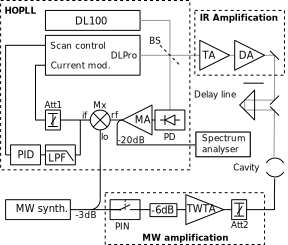
\includegraphics[]{beatexp}
	\caption{Schematic showing how the amplitude modulated laser is produced, locked to the microwave frequency, and how both the laser and microwave fields are delivered to the interaction region. The AM IR laser is generated by overlapping the DL-Pro and DL-100 laser beams on a beamsplitter (BS). One output is amplified and sent to the interaction region. The microwave field is generated by a synthesizer, formed into pulses by the PIN switch and amplified by the Traveling Wave Tube Amplifier (TWTA) before injection into the microwave cavity. The locking of the IR intensity envelope to the microwave field is performed by the Heterodyne Optical Phase Locked Loop (HOPPL).}
	\label{fig:pll}
\end{figure}

Fig.~\ref{fig:pll} shows how the amplitude modulated laser and microwave fields are produced, delivered to the interaction region, and synchronized with a phase locked loop. The 819-nm beam is produced using two external-cavity diode lasers, Toptica DL-100 and DL-Pro lasers. The lasers are tuned such that their frequencies are separated by the microwave frequency, and the two beams are overlapped on a 50:50 beamsplitter (BS). One output from the beamsplitter is directed to a high speed photodetector to detect the microwave frequency beat note and deliver the signal to the phase-locked-loop. The second output from the beamsplitter is directed through an amplification chain and to the interaction region.

The intensity modulation of the laser is locked to the microwave frequency with a heterodyne optical phase-locked-loop (HOPLL). The locking is driven by a "fast" feedback to the current input of the DL-Pro, and a "slow" feedback to the scan input. To produce an error signal, beat note from the photodiode is amplified and mixed with the microwave source to produce an error signal. The error signal is passed through a variable attenuator and then connected to the Current input of the Toptica DL-100, providing a lock between the laser intensity modulation frequency and the microwave field that lasts for several minutes.

To achieve longer lock times, on the order of hours, we use a Toptica PID-110 servo unit to drive the scan input of the DL-Pro. The "fast" current lock described above is primarily lost due to the lasers' drifting out of the range that the DL-100 current input can correct. Low-frequency components of the error signal are processed through the PID-110 and fed to the Scan input, which corrects long term drifts in the amplitude modulation frequency, leaving only high-frequency errors for the "fast" loop to correct.

The second output of the 50:50 beamsplitter produces 30 mW of intensity modulated light, which is passed through a tapered amplifier and a dye amplifier. The Toptica Tapered Amplifier increases the continuous beam power to 800 mW. The dye amplifier is pumped by the 20-ns square pulse picked from the peak of the Nd:YLF laser pulse. We use LDS-819 dissolved in Ethanol as the amplfication medium. The final result is a 20 ns long, 6 $\mu$J pulse of sinusoidally intensity modulated 819-nm light.

Once locked, the AM phase at the BS is constant relative to the MW phase, and their relative phase in the interaction region depends only on the effective path length difference. To adjust the path length of the AM laser beam, after amplification the beam is passed through an optical delay before continuing to the interaction region. This optical delay consists of a retro-reflector mounted to a translation stage, able to extend the path length of the AM laser by several MW wavelengths.

\subsection{\label{cavity} Microwave Apparatus}

A Hittite HMC T-2100 synthesizer tuned to the 15.9-GHz resonance of the microwave cavity is our microwave source. It produces 9 dBm of power, and a splitter diverts half of the power to the microwave mixer to generate the error signal for the PLL. The other half of the signal is formed into 300-ns pulses by a microwave switch, and then amplified by a Hughes 8020H04F traveling-wave-tube-amplifier (TWTA). Between the TWTA and the cavity, there is a 0 to 50 dBm variable attenuator allowing us to control the intensity of the pulse incident on the microwave cavity.

The microwave cavity is a Fabry-Perot cavity composed to two brass spherical mirrors. These mirrors have a radius of curvature of 10 cm and are 10.2 cm in diameter, with an on axis separation of 7.83 cm. The 15.9 GHz resonance is the TEM$_{008}$ mode of the cavity, with a quality factor $Q=3600$. We are able to determine the field inside the cavity with an uncertainty of 15\%. The 300 ns long microwave pulses are injected into the cavity 280 ns before the end of the last laser pulse and are turned off 20 ns after the end of the laser pulse. The microwave field decays with a time constant of vvv ns.

\subsection{\label{fields} Static Fields}

This experiment depends on the detection of long lived Rydberg states close to the ionization limit. To prevent these states from ionizing before detection, we must minimize the persistent static field in the interaction region. We accomplish this by surrounding the interaction region on two sides with the brass microwave cavity mirrors, and on the remaining two sides, top, and bottom with polished aluminum plates. A voltage can be applied independently to each plate or mirror, allowing us to compensate persistent static fields in every direction. We measure the depressed ionization limit (DIL) to minimize stray fields and estimate the residual persistent static field. In this manner, we determine the remaining persistent static field to have a magnitude of 1.5 mV / cm. This results in a DIL of 7 GHz below the the zero field ionization limit. This value for the DIL is constant in all future experiment and discussion in this paper.

To observe phase dependent ionizationin the combined sattic and microwave fields, we apply a pulsed vertical static field to the interaction region during excitation of Rydberg states. We use a two-channel arbitrary waveform generator (AWG) to apply 300-ns square pulses of opposite magnitudes to the top and bottom bias plates. This square pulse is synchronous with the microwave pulse, the leading edge arriving 240-ns before the first laser pulse and the trailing edge arriving 20-ns after the end of the 819-nm laser pulse. Turning off the applied static field minimizes the static field ionization of the high-lying states we wish to observe. 1 $\mu s$ after the final laser pulse, the same AWG applies a voltage to the bottom plate to produce a -0.65 V / cm ionization field, ionizing high-lying states and driving the resulting electrons toward the MCP stack.

\section{\label{results} Results}

The delay scans of Fig.~\ref{fig:fph} show many of the important features of our observations. they are the result of detecting the Rydberg field ionization signal while scanning the time delay $t_0$ with the center frequency of the 819 nm laser tuned 2 GHz above the DIL (5 GHz below the zero-field ionization limit), in the presence of a microwave field of amplitude 4 V/cm and several values of the static field. All of the data reported in this paper were taken with this microwave field. The signal is normalized to the total excitation in the following way. As mentioned in the previous section, to detect the atoms which have survived the static and microwave fields we delay the field ionization pulse by 1 $\mu$s, resulting in the signal $S_{Ryd}$. By reducing the delay to 20 ns results in the signal $S_{total}$, which gives the total number of atoms excited by the laser. The ratio $S$, given by
\begin{equation} \label{eq:norm}
S=S_{Ryd}/S_{total},
\end{equation}
is the normalized signal. Results are shown for $E_{pulse} =$ 0, 7.2, 36.0 and 108.0 mV/cm. the results are in accord with our expectations. First, with zero static field, there is no observed phase dependence, while at 7.2 mV/cm the phase dependent signal is modulated by 5\% of the total excitation, in agreement with the expectation that phase dependent ionization can only be observed at the microwave field frequency when a static field is applied to lift the vertical symmetry of the system. Equally important, when the static field is reversed, to -7.2 mV/cm, the phase dependent modulation reverses sign. As $E_s$ is increased further, both the mean signal and the peak to peak modulation decrease, and the delay at which the detected signal is greatest shifts somewhat at higher pulsed field,
While the addition of a static field in the z direction breaks the symmetry of the two microwave half cycles, a horizontal field should not, and in Fig.~\ref{fig:CircleStatic} we show delay scans analogous to those in Fig.~\ref{fig:fph}. In this case the laser is tuned 14 GHz below the DIL, and the magnitude of the static field is 14 mV/cm. By applying voltages to the bias plates we can apply fields at an angle $\theta$ to the horizontal ($90^{\circ}-\theta$ from the z axis). As shown, there is no modulation with with a horizontal static field, and the observed modulation chages sign as the field is rotated from having a positive to negative z component.

\begin{figure}
	\includegraphics[]{FieldPhase}
	\caption{Rydberg state signal as the phase delay is scanned for various values of $E_S$. The central laser frequency $2\pi\omega_0$ is tuned to 2 GHz above the DIL. The vertical scale is normalized such that 1 is the total number of electrons excited by the 819 nm laser. When no pulsed field is applied, there is no observed phase modulation. As the pulsed field in increased,  phase dependence in the signal grows and then lessens as the total mean signal decreases. Grey shows the experimental data, while the solid sinusoidal curves trace the best fit to Eq.~\ref{eq:modfit}. The traces at + (solid) and -(dashed) 7.2 mV/cm show reversing the static field inverts the amplitude of the phase modulation.}
	\label{fig:fph}
\end{figure}

\begin{figure}
	\includegraphics[width=0.7\textwidth]{CircleDelay}
	\caption{With the central IR frequency $2\pi\omega_o$ tuned to 14 GHz below the DIL, the angle above the horizontal of a 14.4 mV/cm static field ($E_s$) is rotated by applying voltages to vertical and horizontal bias plates. Phase dependence is shown to only emerge when the component of the static field is along the MW and laser polarization is non-zero.}
	\label{fig:CircleDelay}
\end{figure}

It is convenient to quantify these observations by fitting the signal vs. delay to a sinusoidal model:
\begin{equation} \label{eq:modfit}
S = A \cos{(\omega t - \Phi_0)} + S_0
\end{equation}
The frequency is fixed at $\omega/2\pi = 15.9$ GHz, while the amplitude (A), phase offset ($\Phi_0$) and mean signal ($S_0$) are used as fit parameters. We have recorded phase scans such as those of Fig.~\ref{fig:CircleDelay} for several values of $\theta$ on different days, and the results are plotted in Fig.~\ref{fig:CircleStatic}, using the parametrization of Eq.~\ref{eq:modfit}. Each set of data shows the peak to peak modulation crossing zero when $\vec{E}_s$ is nearly horizontal and has a linear relationship with the z-component of the field. A fit to all three sets of data shows modulation is zero at $6.0 \pm 0.9$ degrees below the horizontal, corresponding to a $-1.5 \pm 0.2$ mV/cm z-component of the pulsed field. This is consistent with the $<2$ mV/cm residual static field in the interaction region. As the angle is changed, the amplitude of the phase dependence increases linearly with the component of the pulsed field along the MW and AM laser polarization, which is expected since a static field in the z direction is required to break the symmetry of the system and observe phase dependence.

\begin{figure}
	\includegraphics[]{CircleStatic}
%	\caption{With the central IR frequency $2\pi\omega_o$ tuned to 14 GHz below the DIL, the angle above the horizontal of a 14.4 mV/cm pulsed field is rotated by applying pulsed voltages to vertical and horizontal bias plates. When the pulsed field is perpendicular to the vertical MW and IR polarization, there no phase dependence. The phase dependence grows as $\vec{E}_{pulsed}$ is rotated to have a larger vertical component. The measurement is repeated in three sets, and linear regression on the combined data set shows the peak to peak modulation crosses zero at $6.0 \pm 0.9$ degrees. This corresponds to $\vec{E}_{pulsed} \cdot \hat{z} = 1.5 \pm 0.2$ mV/cm, which is the approximate size of our stray static field.}
	\caption{The measurements shown in Fig.~\ref{fig:CircleDelay} are repeated 3 times on different days. The peak to peak modulation is shown to have a linear dependence on the field angle, or equivalently, the component of the field in the $\hat{z}$ axis, parallel to the MW and IR laser polarization. The zero of the modulation is at $-6.0 \pm 0.9$ degrees, which is compatible with the 1.5 mV/cm persistent static field in the interaction region oriented in along the $\hat{z}$ axis.}
	\label{fig:CircleStatic}
\end{figure}


% \begin{figure}
% 	\includegraphics[width=0.5\textwidth]{ModvsField}
% 	\caption{Mean signal ($S_0$) and peak-to-peak modulation ($2\cdot A$) against applied pulsed static field for excitation laser central frequencies of +2 GHz, -14 GHz, and -30 GHz relative to the DIL. A negative peak-to-peak modulation indicates the greatest Rydberg signal is detected with an optical delay near $\omega t_o = 7\pi/6$, while a negative modulation indicates the detected signal is greatest near $\omega t_o = \pi/6$.}
% 	\label{fig:ModvsField}
% \end{figure}

\begin{figure}
	\includegraphics[]{DILP2}
	\caption{Several signal vs. delay measurements are taken with the central IR frequency $2\pi\omega_o$ tuned to 2 GHz above the DIL at different static field values. The measurements are fit to Eq.~\ref{eq:modfit}, and the peak to peak modulation ($2*A$), mean signal ($S_0$) and phase ($\Phi_0$) of the fits are plotted against $E_S$. At zero field, the mean signal is at a maximum and there is no modulation. We observe that modulation emerges as the magnitude of $E_S$ is increased from zero, reaching a peak at $E_S = 10$ mV/cm. At high field the mean signal and modulation both decay toward zero. The phase is roughly identical for data collected at equal and opposite $E_S$, however a trend of the phase shifting as the magnitude of $E_S$ increases is observed.}
	\label{fig:DILP2}
\end{figure}

With the laser tuned 2 GHz above the DIL we have taken extensive data, of which those shown in Fig.~\ref{fig:fph} are representative. Parameterizing all the data using Eq.~\ref{eq:modfit} yields the plots shown in Fig.~\ref{fig:DILP2}, as expected, 

With $\vec{E}_{pulse}$ parallel to $\hat{z}$, we explore how the fit parameters of Eq~\ref{eq:modfit} change as a function of static field for three tunings of the 819 nm laser relative to the DIL; +2, -14, and -30 GHz. Figs.~\ref{fig:DILP2},~\ref{fig:DILM14}, and~\ref{fig:DILM30} show the peak-to-peak phase dependence in the signal ($2\cdot A$), the mean signal ($S_0$), and the phase ($\Phi_0$) as a function of static field. For all three laser tunings, the mean signal behaves as expected. The signal is largest when there is no static field applied, and the high lying states we detect are longer lived. As the magnitude of the applied static field increases, mean signal monotonously decreases as the high lying states are more likely to ionize. The further below the DIL the central frequency of the excitation laser is tuned, the more slowly $S_0$ drops off with field.

\begin{figure}
	\includegraphics[]{DILM14}
	\caption{Several measurements are taken as described in Fig.~\ref{fig:DILP2}, however with the central IR frequency $2\pi\omega_o$ tuned to 14 GHz below the DIL. At zero field, we again observe the signal is at a maximum and there is no modulation. Modulation emerges with the opposite sign as when the laser is tuned above the limit, as in Fig.~\ref{fig:DILP2}, as the magnitude of $E_S$ is increased from zero. Peak modulation is reached at $E_S = \pm 12$ mV/cm. The modulation then crosses zero at $E_S = \pm 25$ mV/cm and changes sign. At high field the mean signal and modulation again decay to zero with the same sign as seen above the limit. The trend of the phase shifting as the magnitude of $E_S$ increases is again observed.}
	\label{fig:DILM14}
\end{figure}

\begin{figure}
	\includegraphics[]{DILM30}
	\caption{Several measurements are taken as described in Figs.~\ref{fig:DILP2} and~\ref{fig:DILM14}, with the central IR frequency $2\pi\omega_o$ tuned to 30 GHz below the DIL. Modulation does immediately emerge as seen at 2 GHz above and 14 GHz below the DIL. Rather, there is a "turn on" field of $~ E_S = \pm 20$ mV/cm. Above this field, the modulation behaves similarly to measurements at 14 GHz below the DIL shown in Fig.~\ref{fig:DILM14}, with peak modulation occurring at $E_S = \pm 40$ mV/cm, and the zero crossing occurring at $\pm 65$ mV/cm.}
	\label{fig:DILM30}
\end{figure}

The observed behavior of the peak-to-peak modulation is more complex. Fig.~\ref{fig:DILP2} shows observations with a laser tuning 2 GHz above the DIL. As shown in Fig.~\ref{fig:fph}, at zero static field the symmetry of the system is not lifted and we cannot observe phase dependence. As the static field magnitude is increased phase dependence quickly emerges, reaching the maxima of peak-to-peak amplitude at $E_s = \pm 10$ mV/cm. As the magnitude of the static field is further increased, the average signal approaches zero, as does the modulation. In these figures, the peak to peak amplitude ($2 \cdot A$) is positive if $\Phi_0 \approx 7\pi/6$, and negative if $\Phi_0 \approx \pi/6$. Because the applied static field is the only parameter lifting the vertical symmetry, reversing the static field inverts the modulation. This shows in the peak-to-peak modulations at opposite applied static fields being approximately equal and opposite, corresponding to peak signal occurring at optical delays separated by $\Delta \Phi_0 = \pi$.

In Fig.~\ref{fig:DILM14}, showing the laser tuned 14 GHz below the DIL, the behavior is more complex. Like the DIL + 2 GHz case, the amplitude of the peak to peak signal quickly increases as the pulsed field is increased from zero, reaching a peak near $\pm$10 mV/cm. However, the modiulation is inverted relative to that shown in Fig.~\ref{fig:DILP2}. As the magnitude of the static field is increased, the modulation falls, crossing through zero at $\pm$25 mV/cm, reaching a peak at $\pm$50 mV/cm and then decreasing as the amplitude of the field is further increased. For fields inexcess of $\pm$25 mV/cm the modulation has the same sign as that of Fig~\ref{fig:DILP2}.

Finally, Fig.~\ref{fig:DILM30} shows the case for the laser tuned to DIL - 30 GHz. It resembles the DIL - 14 GHz case of Fig.~\ref{fig:DILM14}, except that there is no modulation for a finite region around zero static field. The modulation does not appear until the static field reaches $\pm$ 20 mV/cm. appears to turn on at a non-zero pulsed field. Rather than immediately growing as the pulsed field is increased, the modulation doesn't start growing until $E_s = \pm 20$ mV/cm. We attribute this to only a small window of phases allow either uphill or downhill to gain enough energy to ionize at small pulsed field. Thus the modulation doesn't start to rapidly increase until the depressed potential barrier seen by downhill electrons is pushed closer to $W_0$, at which point the system starts to more closely resemble Fig.~\ref{fig:DILM14}.

\section{\label{sec:disc} Comparison to Computational Model}

To provide insight into the observed phase dependence in the number of detected atoms as well as the phase reversal observed when the laser is tuned below the DIL we have constructed a two-dimensional model of a classical Rydberg electron moving in the combined Coulomb, static, and microwave (mw) fields. Expressed in atomic units, the equation of motion is:
\begin{align*}
\ddot{\vec{r}} & = -\vec{E}_{coul}(\vec{r}) - \vec{E}_{s}(t) - \vec{E}_{mw}(t) \\
 & = -\frac{1}{r^2} \cdot \hat{r} - \Theta_s(t) \cdot E_{s} \cdot \hat{z} - \Theta_{mw}(t) \cdot E_{mw} \sin{(\omega t + \phi_0)} \cdot \hat{z}
\end{align*}
$\Theta_s$ and $\Theta_{mw}$ are envelopes describing the square wave turning off the static  field and the exponential ring-down of the MW field. Explicitly,
\begin{align*}
\Theta_s(t \leq t_{off}) & = 1 & \Theta_{mw}(t \leq t_{off}) & = 1 \\
\Theta_s(t > t_{off}) & = 0 & \Theta_{mw}(t > t_{off}) & = e^{-(t-t_{off})/\tau_{mw}}.
\end{align*}
The microwave field amplitude is 4 V/cm, the frequency is 15.9 GHz, the microwave and static fields are turned off at $t_0 = 20$ ns, and $\tau_{mw} = 80$ ns. The electron is launched at time $t=0$ starting from the periapsis of the highly elliptical Rydberg orbit with an initial energy $W_0$ and initial angular momentum $l_0 = \sqrt{3 \cdot (3+1)}$, corresponding to an $f$ state. the electron's orbit lies in the x-z plane, and initially it is in an elliptical orbit with its semi-major axis along the the +z or -z axis. In Fig.~\ref{fig:udo} we show the beginnings of two trajectories, A and B, which are initially on elliptical orbits. If the static field $E_s$ is in the +z direction, as shown, an electron launched on trajectory (a) is reflected back toward the ion by the static field, and we label it an "uphill" trajectory. An electron launched on trajectory (b) is a "downhill" trajectory. Both trajectories shown in Fig.~\ref{fig:udo} have angular momentum in the +y direction. As expected from the symmetry of the problem, the results we obtain are unchanged when the sign of the angular momentum is reversed.

\begin{figure}
	\includegraphics[]{UDO}
	\caption{Schematic showing the beginning of "downhill" (B) and "uphill" (A) electron orbits in the 2 dimensional simulation, with the ion core at $(x, z) = (0, 0)$. Given initial radius and velocity $r_0$ and $v_0$, downhill electrons are launched from $(0, -r_0)$, with velocity in the $-\hat{x}$ direction. Uphill electrons are launched from $(0, +r_0)$ with velocity along $+\hat{x}$. Both orbits shown have angular momentum aligned in the $+\hat{y}$ direction. In the absence of a static field, bound electrons make highly elliptical orbits with the semi-major axis along the z-axis. The field $E_S$ applies a force in the $+\hat{z}$ direction on electrons during their orbits.}
	\label{fig:udo}
\end{figure}

For computation, the vector equations are expressed in terms of Cartesian coordinates \{x,y,z\}. Including the initial conditions, the system of ordinary differential equations to integrate is:
\begin{align*}
x(0) & = 0 & z(0) & = \pm r_0 \\
\dot{x}(0) & = \pm v_0 & \dot{z}(0) & = 0 \\
\ddot{x} & = -\frac{x}{(x^2 + z^2)^{3/2}} & \ddot{z} & = -\frac{z}{(x^2 + z^2)^{3/2}} - \Phi_s(t) \cdot E_s \\
 & & & \quad \quad - \Phi_{mw}(t) \cdot E_{mw} \cdot \sin{(\omega t + \phi_0)}
\end{align*}

For each initial electron energy $W_0$ and static field $E_s$, electrons are launched at 200 microwave phases $\phi_0$ between 0 and $2\pi$, in the "uphill" and "downhill" directions. The equations of motion are integrated until the MW field has decayed for 5 times the decay constant, that is until  $t=t_{off} + 5\tau_{MW}$. After this integration time, the final energy, $W_f = 1/2 v_f^2 - 1/r_f$, of the electron is recorded.

An electron with a positive final energy escapes from the ion, while those with negative final energies are bound and detected. The detected signal as a function of phase is convolved with the intensity envelope of the laser to produce a simulated signal. We assume the laser intensity profile to be given by Eq.~\ref{eq:modfit}. The calculated signals are normalized in the same way as the experimental data. To provide the maximum insight into the origin of the observed signals we treat the uphill and downhill electrons separately, then add them to produce the calculated signal. 
In Fig.~\ref{fig:2DW0} we show the results for $W_0 =$ 0, 36, and 100 mV/cm. These calculations should mimic the experimental results shown in Fig.~\ref{fig:DILP2}. As expected, with $E_s=0$ there are equal modulations in the electrons ejected uphill, the +z direction, and downhill, the -z direction. The maximum in the uphill (downhill) signal occurs at $\phi_0=\pi/6$ ($7\pi/6$), the phase at which the microwave field removes the most energy from an uphill (downhill) electron. Since the modulations are $\pi$ out of phase, they cancel in the detected signal. In a static field of 36 mV/cm most of the downhill electrons leave, with a few surviving at $\phi_0=7\pi/6$, the phase at which the microwave field removes the maximum amount of energy from a downhill electron. More uphill electrons survive as bound atoms at all phases, but they are much more likely to survive if $\phi_0=\pi/6$, the phase at which the microwave field extracts the most energy from an uphill electron. Adding the uphill and downhill signals yields a total signal with a peak at $\phi_0=\pi/6$. When the static field is increased to 100 mV/cm no electrons ejected downhill result in bound atoms; the entire detected signal is due to electrons launched uphill. Irrespective of the static field the maximum number of bound atoms from uphill electrons occurs at $\phi_0=\pi/6$. These calculations, which are in agreement with the model of Shuman et al., are why we fixed the phase of the maximum experimental signals at $\phi_0=\pi/6$.

\begin{figure}
	\includegraphics[]{Sim0}
	\caption{Calculated observed signal from our 2 dimensional model, with initial energy $W_0 = 0$ GHz. The contributions from downhill and uphill electrons are in orange (dotted) and blue (dashes), respectively, with the total expected signal in Green. At $E_{pulse} = 0$ mV/cm, uphill and downhill signals have opposite phase dependence, resulting in a flat total signal. As the field increases, ionization of downhill electrons depresses their mean signal and modulation, and the total signal becomes dominated by contributions from uphill electrons.}
	\label{fig:2DW0}
\end{figure}

A surprising aspect of our data is the sign reversal of the modulation with increasing static field when the laser is tuned below the DIL, as seen in Figs.~\ref{fig:DILM14} and \ref{fig:DILM30}. Fig.~\ref{fig:2DW20} shows the results for $W_0 = -20$ GHz and $E_s = 0, ~7.2, ~100$ mV/cm. As for $W_0=0$, when $E_s=0$ there is no modulation when the uphill and downhill signals are summed. When $E_s=$7.2 mV/cm the maximum in the number of bound atoms detected occurs at $\phi_0=7\pi/6$, not $\pi/6$. The calculated signal exhibits the same phase reversal seen in the experimental data of Figs.~\ref{fig:DILM14} and \ref{fig:DILM30}. Examining the uphill and downhill electron contributions separately shows the origin of the reversal. At $E_s = 7.2$ mV/cm many of the uphill electrons are left as bound electrons for all phases, with only a slight dependence on $\phi_0$. While fewer of the downhill electrons are left bound, the dependence on $\phi_0$ is much ore pronounced, leading to a peak in the total detected signal at $\phi_0=7\pi/6$. When the static field is raised to 100 mV/cm essentially all the downhill electrons leave the ion, and the uphill electrons, which are most likley to remain bound when $\phi_0=\pi/6$, constitute almost the entire signal. In the presence of the larger static field the tuning slightly below the limit becomes equivalent to tuning to the limit in any static field.

\begin{figure}
	\includegraphics[]{SimM20}
	\caption{Calculated observed signal from our 2 dimensional model, with initial energy $W_0 = -20 GHz$. Downhill and uphill signals are in orange (short-dashes) and blue (long dashes), respectively, with total signal in green. As in Fig.~\ref{fig:2DW0}, at $E_{pulse} = 0$ mV/cm, the uphill and downhill signals result in a flat total signal. At $E_{pulse} = 7.2$ mV/cm, the downhill signal is diminished, but the total phase dependence increases. The total signal shows a phase dependence shifted by $\pi$ from the small field signal for $W_0 = 0 GHz$ in Fig.~\ref{fig:2DW0}. At $E_{pulse} = 100$ mV/cm, downhill electrons almost all ionize, and the uphill signal dominates the total signal.}
	\label{fig:2DW20}
\end{figure}

In sum, The model shows both the origins of the phase dependence and its unexpected reversal encountered when the laser is tuned below the DIL.

\section{\label{sec:conc} Conclusions}

\emph{EMPTY}

%\bibliography{basename of .bib file}

\end{document} 